\documentclass[11pt,a4paper]{article}

% =================================================
% Packages
% =================================================
\usepackage[T1]{fontenc}
\usepackage[utf8]{inputenc}
\usepackage{lmodern}

\usepackage{amsmath, amssymb, amsfonts, amsthm}
\usepackage{mathtools}
\usepackage{physics}
\usepackage{bm} % bold math symbols (vectors/matrices)
\usepackage{microtype}

\usepackage{graphicx}
\usepackage{booktabs}
\usepackage{hyperref}
\usepackage{geometry}
\usepackage{natbib}
\usepackage{enumitem}
\usepackage{caption}
\usepackage{subcaption}

\usepackage{algorithm}
\usepackage{algorithmic}

\usepackage{tikz}
\usetikzlibrary{arrows.meta, calc, positioning, patterns, shapes.geometric}

\usepackage{dsfont} % indicator function

\geometry{margin=1in}
\hypersetup{colorlinks=true, linkcolor=blue, citecolor=blue, urlcolor=blue}

% =================================================
% Notation & macros (strict conventions)
% =================================================
% Scalars: italic (default), e.g. x, \epsilon
% Vectors: bold lowercase, e.g. \mathbf{x}

% CACIS / Fenchel--Young convenience
\newcommand{\valpha}{\bm{\alpha}} % simplex variable
\newcommand{\ve}{\mathbf{e}}      % canonical basis
\newcommand{\FW}{\mathrm{FW}}     % Frank--Wolfe
\newcommand{\CACIS}{\textsc{CACIS } }
\newcommand{\FY}{\mathrm{FY}}

% Matrices: bold uppercase, e.g. \mathbf{C}
% Random variables: uppercase, e.g. X
% Sets/spaces: calligraphic, e.g. \mathcal{X}
% Probability simplex: \Delta^K

% Vectors
\newcommand{\vx}{\mathbf{x}}
\newcommand{\vy}{\mathbf{y}}
\newcommand{\vp}{\mathbf{p}}
\newcommand{\vq}{\mathbf{q}}
\newcommand{\vz}{\mathbf{z}}
\newcommand{\vone}{\mathbf{1}}
\newcommand{\vpi}{\bm{\pi}} % transport plan (bold greek)



% Matrices
\newcommand{\mC}{\mathbf{C}} % cost matrix
\newcommand{\mK}{\mathbf{K}} % Gibbs kernel
\newcommand{\mM}{\mathbf{M}} % CACIS kernel matrix
\newcommand{\mP}{\mathbf{P}}
\newcommand{\mQ}{\mathbf{Q}}
\newcommand{\mI}{\mathbf{I}}
\newcommand{\mV}{\mathbf{V}} % value matrix

% Sets / numbers
\newcommand{\R}{\mathbb{R}}

% Expectations / indicators
\newcommand{\E}{\mathbb{E}}
\newcommand{\Ind}{\mathds{1}}

% Named quantities
\newcommand{\KL}{\mathrm{KL}}
\newcommand{\OT}{\mathrm{OT}}
\newcommand{\Sink}{\mathrm{Sink}}
\newcommand{\softmax}{\mathrm{softmax}}

\DeclareMathOperator*{\argmin}{arg\,min}
\DeclareMathOperator*{\argmax}{arg\,max}
\DeclareMathOperator{\sign}{sign}
\DeclareMathOperator{\diag}{diag}

% =================================================
% Theorems (for scientific style)
% =================================================
\newtheorem{proposition}{Proposition}
\newtheorem{remark}{Remark}

% =================================================
% Metadata
% =================================================
\title{\textbf{Beyond Cross-Entropy:\\
Cost-Aware Decision-Theoretic Learning\\with Optimal Transport for Classification}\\[1mm]
}

\author{
Warith Harchaoui \\
\small Head of AI, NEXTON
\and
Laurent Pantanacce \\
\small AI Business Manager, NEXTON
}

\date{January 2026}

\begin{document}
\maketitle

\begin{abstract}
Classification systems rarely operate in isolation: predictions trigger decisions with
asymmetric and context-dependent consequences. Yet the dominant training objective in
modern classifiers---cross-entropy (negative log-likelihood)---implicitly treats all
misclassifications as equally undesirable and ignores the geometry induced by
business or semantic values on the label set.
This report develops a decision-theoretic and geometric view of classification,
and shows how \emph{Optimal Transport} (OT) and \emph{entropically-regularized OT}
(Sinkhorn losses) provide principled, differentiable surrogates for real-world
decision costs. We clarify the relationship to cross-entropy, provide algorithms,
and offer practical guidelines for cost design and model training.
We introduce \CACIS (Cost-Aware Classification with Informative Selection), a Fenchel--Young loss induced by a Sinkhorn/OT regularizer, which injects the cost geometry directly into training and yields a differentiable, decision-aligned objective.
\end{abstract}

\tableofcontents
\newpage

% =================================================
\section{Notation and problem setting}
% =================================================

Let $\mathcal{X}$ be an input space and $\mathcal{Y}=\{1,\dots,K\}$ a finite label set.
A classifier produces a predictive distribution $\vp(\vx)\in\Delta^K$, where
\[
\Delta^K \coloneqq \Bigl\{\vp\in\R^K_{\ge 0}:\textstyle\sum_{k=1}^K p_k = 1\Bigr\}
\]
is the probability simplex.
We write $Y$ for a random label and $X$ for a random input, with joint distribution
$\mathbb{P}$ over $\mathcal{X}\times\mathcal{Y}$.
A parametrized model (e.g.\ a neural network) outputs logits $\vz_\theta(\vx)\in\R^K$
and probabilities $\vp_\theta(\vx)=\softmax(\vz_\theta(\vx))$.
Unless stated otherwise, vectors are bold lowercase (e.g.\ $\vx$) and matrices bold uppercase (e.g.\ $\mC$).

\paragraph{From prediction to decision.}
A \emph{decision rule} maps $\vp$ to an action/decision $a\in\mathcal{A}$.
In standard $K$-class classification with \emph{hard} decisions, $\mathcal{A}=\mathcal{Y}$.
More generally, actions can represent interventions, resource allocations, or abstentions.
We focus on the common case $\mathcal{A}=\mathcal{Y}$ to keep notation minimal, while the framework extends directly to richer action spaces.

\paragraph{Costs and values.}
We encode operational consequences by a cost matrix $\mC\in\R^{K\times K}_{\ge 0}$,
where $C_{ij}$ is the cost incurred when the true class is $i$ but we decide $j$.
In business contexts, one often starts from a value matrix $\mV$ (profits, utilities) and sets
$C_{ij}$ as \emph{regret} relative to the optimal action under truth $i$, e.g.\
\[
C_{ij}=V_{i i^\star}-V_{ij},
\qquad
i^\star\in\argmax_j V_{ij}.
\]
This is useful because it makes ``zero cost'' correspond to the best decision under the realized outcome. Most of the time, we would have $i^\star = i$ so that $C$ would have zeros on its diagonal.

% =================================================
\section{Introduction}
% =================================================

Geometry is the opportunity to inject cost, value, and business semantics
directly into the learning objectives of corporate AI systems.
While modern classifiers are typically trained using cross-entropy,
this objective implicitly assumes uniform misclassification costs
and a trivial geometry on the label space.



\paragraph{A concrete contribution: \CACIS.}
Beyond the general OT/Sinkhorn viewpoint, we propose a concrete training objective, \CACIS, formulated as a Fenchel--Young loss generated by a Sinkhorn-based regularizer. \CACIS keeps the probabilistic benefits of cross-entropy (smooth gradients, calibration) while replacing the ``flat'' label geometry by the task geometry encoded in the cost matrix $\mC$.
This report develops a decision-theoretic and geometric view of classification.
We show how costs induce a non-trivial geometry on labels,
how cross-entropy arises as a special and degenerate case,
and how Optimal Transport (OT) and entropically regularized OT (Sinkhorn losses)
provide principled, differentiable surrogates for real-world decision costs.

Modern machine learning systems are evaluated within socio-technical pipelines:
a model output triggers a decision, which triggers a downstream outcome,
often with non-symmetric and context-dependent consequences.
Accuracy and cross-entropy are convenient proxies, but they can be misaligned with
the \emph{value} delivered (or lost) by the overall system.

This report argues that:
\begin{itemize}[leftmargin=*]
    \item classification is fundamentally a \emph{decision problem} under uncertainty;
    \item costs induce a non-trivial geometry on labels (a ``ground metric'');
    \item learning objectives should align with \emph{expected cost} or \emph{expected value},
          not only with proxy measures of correctness.
\end{itemize}

% \paragraph{Suggested figure (TikZ).}
% Figures~\ref{fig:pipeline_accuracy} and \ref{fig:pipeline_cost} contrast a classical accuracy-based pipeline with a
% decision-theoretic pipeline.

\begin{figure}[h]
\centering
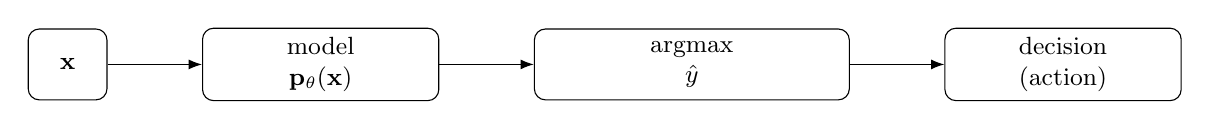
\begin{tikzpicture}[node distance=12mm, >=Latex, font=\small]
\node[draw, rounded corners, align=center, minimum width=10mm, minimum height=9mm] (x) {$\vx$};
\node[draw, rounded corners, align=center, minimum width=30mm, minimum height=9mm, right=of x] (model) {model\\$\vp_\theta(\vx)$};
\node[draw, rounded corners, align=center, minimum width=40mm, minimum height=9mm, right=of model] (argmax) {argmax\\$\hat{y}$};
\node[draw, rounded corners, align=center, minimum width=30mm, minimum height=9mm, right=of argmax] (decision) {decision\\(action)};
\draw[->] (x) -- (model);
\draw[->] (model) -- (argmax);
\draw[->] (argmax) -- (decision);
\end{tikzpicture}
\caption{Accuracy-based pipeline using only $\hat{y}$.}
\label{fig:pipeline_accuracy}
\end{figure}

\begin{figure}[h]
\centering
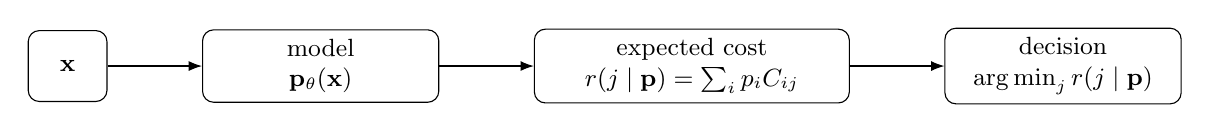
\begin{tikzpicture}[node distance=12mm, >=Latex, font=\small]
\node[draw, rounded corners, align=center, minimum width=10mm, minimum height=9mm] (x2) {$\vx$};
\node[draw, rounded corners, align=center, minimum width=30mm, minimum height=9mm, right=of x2] (model2) {model\\$\vp_\theta(\vx)$};
\node[draw, rounded corners, align=center, minimum width=40mm, minimum height=9mm, right=of model2] (risk) {expected cost\\$r(j\mid \vp)=\sum_i p_i C_{ij}$};
\node[draw, rounded corners, align=center, minimum width=30mm, minimum height=9mm, right=of risk] (dec2) {decision\\$\argmin_j r(j\mid\vp)$};
\draw[->] (x2) -- (model2);
\draw[->] (model2) -- (risk);
\draw[->] (risk) -- (dec2);
\end{tikzpicture}
\caption{Cost-aware decision-theoretic pipeline using $\vp$ and $\mC$.}
\label{fig:pipeline_cost}
\end{figure}

% =================================================
\section{Related Work}
% =================================================

This work sits at the intersection of statistical decision theory,
cost-sensitive learning, and geometric approaches to loss design.
We review the most relevant strands of literature and clarify
how the present contribution relates to and departs from them.

\subsection{Decision theory and cost-sensitive classification}

The formulation of prediction as a decision problem under uncertainty
is classical in statistical decision theory.
Given a loss or cost function defined over pairs of true outcomes and actions,
the Bayes-optimal decision rule minimizes expected risk
\citep{berger1985statistical}.
In the classification setting, this yields decision rules of the form
\[
\hat{y}(\vp) = \argmin_j \sum_i p_i C_{ij},
\]
which depend on the full predictive distribution rather than solely
on the most likely class.

In machine learning, this perspective appears under the umbrella of
\emph{cost-sensitive learning}, where misclassification costs are asymmetric,
class-dependent, or application-specific.
Common techniques include class reweighting,
threshold adjustment, or post-hoc decision rules.
However, many such approaches treat costs as scalar weights
and do not explicitly model relationships between incorrect labels.
As a result, they fail to capture the geometric structure
induced by realistic cost matrices.

Our work emphasizes that costs are not merely weights,
but define a geometry on the label space
that should be respected both at training and decision time.

\subsection{Proper scoring rules and cross-entropy}

Cross-entropy plays a central role in modern classification
because it arises as the negative log-likelihood of a categorical model
and as a strictly proper scoring rule.
Proper scoring rules incentivize truthful probability estimation
by ensuring that the expected score is minimized by the true distribution
\citep{gneiting2007strictly}.

From an information-theoretic perspective,
cross-entropy minimization is equivalent to minimizing
the expected Kullback--Leibler divergence
between the true conditional distribution and model predictions.
This induces a specific information geometry on the probability simplex,
in which all incorrect labels are treated as equally distant.

While this geometry is appropriate when the objective
is probability estimation under uniform misclassification costs,
it becomes inadequate when different errors have different
operational or semantic meanings.
Weighted cross-entropy partially addresses class imbalance,
but does not introduce a meaningful geometry between labels,
nor does it encode pairwise or hierarchical relationships.

\subsection{Surrogate losses and margin-based methods}

The replacement of the 0--1 loss by convex surrogate losses
is a cornerstone of statistical learning theory.
In binary classification, hinge loss (support vector machines)
and logistic loss (logistic regression)
are the two canonical convex relaxations of the step loss.
Both are classification-calibrated
and yield Bayes-consistent classifiers under appropriate conditions
\citep{bartlett2006convexity}.

In multiclass settings, several extensions of margin-based losses
have been proposed, including multiclass hinge losses
and softmax-based cross-entropy.
However, these constructions typically assume a flat label space
and uniform misclassification costs.
They do not naturally account for graded notions of error,
such as semantic similarity or operational proximity between classes.

In this sense, cross-entropy should be understood
not as a universally appropriate objective,
but as a particular smooth relaxation of the step loss
associated with a degenerate cost geometry.

\subsection{Optimal Transport and geometric losses}

Optimal Transport (OT) provides a principled framework
for comparing probability distributions under a prescribed ground cost
\citep{villani2008optimal}.
Recent advances in entropic regularization
and the Sinkhorn algorithm
have made OT differentiable and computationally efficient,
leading to widespread adoption in machine learning
\citep{cuturi2013sinkhorn, benamou2015iterative}.

A comprehensive treatment of OT theory, algorithms,
and applications in data science
is given by \citet{peyre2019computational}.
Entropically regularized OT has been applied to
domain adaptation, generative modeling,
representation learning, and clustering.

Sinkhorn divergences were introduced
to correct the bias of entropic OT
and to interpolate smoothly between
Wasserstein distances and kernel-based discrepancies
\citep{genevay2018learning, feydy2019interpolating}.
Their statistical properties,
including sample complexity and convergence rates,
have been studied in detail
\citep{genevay2019sample}.

\subsection{OT as a loss for supervised learning}

The use of OT as a loss function in supervised learning
has gained attention in recent years.
\citet{mensch2019geometric} introduce \emph{geometric losses}
for learning with structured output spaces,
showing that OT-based losses naturally encode task-specific geometry
and yield well-behaved gradients.

In classification, OT-based losses have been used
to incorporate label similarity,
hierarchical relationships,
and semantic distances between classes.
Compared to cross-entropy,
these losses penalize mistakes in a graded manner
consistent with domain knowledge,
rather than collapsing all errors into a single category.

The present work builds on these insights
but emphasizes a decision-theoretic interpretation:
the cost matrix underlying OT is not merely a similarity heuristic,
but a formal encoding of operational regret.
This perspective provides a direct and explicit bridge
between business objectives, decision rules,
and learning objectives.

\subsection{Software and practical adoption}

The practical adoption of OT-based methods
has been facilitated by the availability
of robust and efficient software libraries.
The \texttt{POT} (Python Optimal Transport) library
provides state-of-the-art implementations
of OT, Sinkhorn, and related algorithms,
and is widely used in both research and industry
\citep{flamary2021pot, flamary2024pot}.

These tools make it feasible
to integrate OT-based losses
into modern deep learning pipelines,
enabling end-to-end training
with cost-aware and geometry-aware objectives.

\subsection{Positioning of the present work}

In contrast to approaches that treat costs as weights
or similarities as heuristics,
this work advocates a unified view:
\begin{itemize}
\item costs encode regret relative to optimal decisions,
\item regret induces a geometry on the label space,
\item Optimal Transport provides the appropriate mathematical machinery
      to compare predictive distributions in that geometry.
\end{itemize}

By making the connection between decision theory,
geometry, and learning objectives explicit,
this paper aims to provide both a conceptual framework
and practical guidance for deploying
cost-aware machine learning systems
in real-world, decision-critical settings.

% =================================================
\section{Cross-Entropy Revisited}
% =================================================

Cross-entropy is the dominant training objective for probabilistic classifiers.
Its prevalence is not accidental: it can be derived from several distinct and
mutually consistent perspectives.
In this section, we revisit cross-entropy through three complementary lenses:
(i) maximum likelihood estimation,
(ii) expectation of Kullback--Leibler divergence,
and (iii) smooth relaxation of the 0--1 loss.
Together, these derivations clarify both its strengths and its structural limitations
for cost-sensitive decision problems.

% -------------------------------------------------
\subsection{Cross-entropy as negative log-likelihood}
% -------------------------------------------------

\paragraph{Probabilistic model.}
Let $(X,Y)$ be random variables with joint distribution $\mathbb{P}$,
where $Y\in\mathcal{Y}=\{1,\dots,K\}$.
A parametric classifier with parameters $\theta$ models the conditional distribution
\[
\mathbb{P}_\theta(Y = k \mid X = \vx) = p_{\theta,k}(\vx),
\qquad
\vp_\theta(\vx) \in \Delta^K.
\]

Given an i.i.d.\ dataset $\{(\vx_n, y_n)\}_{n=1}^N$,
the conditional log-likelihood is
\[
\ell(\theta) = \sum_{n=1}^N \log p_{\theta,y_n}(\vx_n).
\]

\paragraph{Maximum likelihood estimation.}
Maximum likelihood estimation (MLE) selects parameters
\[
\hat{\theta} = \argmax_\theta \ell(\theta),
\]
or equivalently minimizes the negative log-likelihood
\[
\mathcal{L}_{\mathrm{NLL}}(\theta)
=
-\frac{1}{N} \sum_{n=1}^N \log p_{\theta,y_n}(\vx_n).
\]

When labels are encoded as one-hot vectors $\vy_n = e_{y_n}$,
this loss can be written as
\[
\mathcal{L}_{\mathrm{CE}}(\theta)
=
-\frac{1}{N}
\sum_{n=1}^N
\sum_{k=1}^K
y_{n,k} \log p_{\theta,k}(\vx_n),
\]
which is precisely the \emph{cross-entropy} between the empirical label distribution
and the model predictions.

\paragraph{Interpretation.}
From this viewpoint, cross-entropy is statistically natural:
it is the unique objective that makes the model assign high probability
to the observed labels.
However, this derivation is agnostic to downstream decisions and costs:
it optimizes \emph{probability estimation}, not \emph{decision quality}.

% -------------------------------------------------
\subsection{Cross-entropy as expected KL divergence}
% -------------------------------------------------

\paragraph{Population-level objective.}
Let $\mathbb{P}(Y=\cdot \mid X=\vx)$ denote the true conditional distribution.
The expected negative log-likelihood can be written as
\[
\E_{X,Y}\bigl[-\log p_{\theta,Y}(X)\bigr]
=
\E_X \left[
\sum_{k=1}^K
\mathbb{P}(Y=k\mid X)
\bigl(-\log p_{\theta,k}(X)\bigr)
\right].
\]

\paragraph{Decomposition via KL divergence.}
For each $\vx$, define the true conditional distribution
$\vq(\vx) = \mathbb{P}(Y=\cdot\mid X=\vx)$.
Then
\begin{align}
\E_{Y\mid X=\vx}\!\left[-\log p_{\theta,Y}(\vx)\right]
&= H(\vq(\vx)) + \KL\!\bigl(\vq(\vx)\,\|\,\vp_\theta(\vx)\bigr).
\end{align}
Taking expectation over $X$, we obtain
\begin{align}
\E_{X,Y}\bigl[-\log p_{\theta,Y}(X)\bigr]
&=
\E_X\bigl[H(\vq(X))\bigr]
+
\E_X\bigl[\KL(\vq(X)\,\|\,\vp_\theta(X))\bigr].
\end{align}

\paragraph{Consequence.}
Since the entropy term does not depend on $\theta$,
minimizing cross-entropy is equivalent to minimizing the expected KL divergence
between the true and predicted conditional distributions.

\paragraph{Geometric interpretation.}
KL divergence induces an information geometry on the probability simplex $\Delta^K$.
This geometry:
\begin{itemize}
\item is asymmetric,
\item strongly penalizes missing mass on true labels,
\item ignores semantic or operational relationships between incorrect labels.
\end{itemize}
Thus, cross-entropy encourages \emph{distributional fidelity},
but with respect to a geometry that treats all misclassifications as equally distant.

% -------------------------------------------------
\subsection{Cross-entropy as a smooth relaxation of the step loss}
% -------------------------------------------------

\paragraph{Binary classification and the step loss.}
We begin with the binary classification setting
$\mathcal{Y}=\{-1,+1\}$.
Let $f_\theta(\vx)\in\R$ denote a real-valued score (logit),
and consider the hard decision rule
\[
\hat{y} = \sign\!\bigl(f_\theta(\vx)\bigr).
\]
Under uniform misclassification costs,
the loss incurred by a hard decision is the 0--1 loss
\[
\ell_{\mathrm{0\text{-}1}}(y,f) = \Ind\{y f \le 0\}.
\]
As a function of the signed margin $y f$,
this loss is a \emph{step function}:
it equals $1$ for incorrect predictions ($y f \le 0$)
and $0$ for correct ones ($y f > 0$).

The Bayes-optimal classifier under this loss
predicts the most likely label,
and the corresponding risk minimization problem
is well-defined but computationally intractable,
as the step loss is discontinuous and non-convex.

\paragraph{From step loss to convex surrogates.}
To enable gradient-based optimization,
the step loss is replaced by a convex surrogate
that upper-bounds it while preserving its ordering.
Two canonical relaxations are widely used.

\paragraph{Hinge loss (SVM).}
The hinge loss replaces the step by a piecewise linear,
convex function:
\[
\ell_{\mathrm{hinge}}(y,f)
=
\max(0,\,1 - y f).
\]
This loss enforces a \emph{hard margin}:
predictions are only penalized if the margin $y f$ is smaller than $1$.
Geometrically, the hinge loss encourages separation with a safety buffer,
but does not define a probabilistic model.
Gradients vanish once the margin constraint is satisfied.

\paragraph{Logistic loss (cross-entropy).}
The logistic loss provides a smooth alternative:
\[
\ell_{\mathrm{logistic}}(y,f)
=
\log\bigl(1 + e^{-y f}\bigr).
\]
Unlike the hinge loss, it is everywhere differentiable
and strictly convex.
As $y f \to -\infty$, the loss grows linearly,
while as $y f \to +\infty$, it decays exponentially.

This loss corresponds exactly to the negative log-likelihood
of a Bernoulli model with
\[
p_\theta(y=1\mid \vx)=\sigma\!\bigl(f_\theta(\vx)\bigr),
\]
where $\sigma$ is the logistic sigmoid.
Thus, minimizing logistic loss is equivalent to
maximum likelihood estimation in a probabilistic model.

\paragraph{Comparison of relaxations.}
Both hinge and logistic losses are convex upper bounds
of the step loss, but they encode different inductive biases:
\begin{itemize}
\item hinge loss enforces margins but ignores probability calibration,
\item logistic loss yields calibrated probabilities and smooth gradients,
\item both assume symmetric misclassification costs.
\end{itemize}

\paragraph{Expected step loss and probabilistic relaxation.}
For a fixed true label $y=1$,
the expected 0--1 loss under a predictive probability $p$
is
\[
\mathcal{L}_{\mathrm{step}}(p) = 1 - p.
\]
Cross-entropy replaces this linear penalty
with a logarithmic barrier:
\[
1 - p
\quad \longrightarrow \quad
-\log p.
\]
This transformation preserves ordering,
penalizes confident but wrong predictions infinitely,
and yields informative gradients even near the decision boundary.

\paragraph{Extension to multiclass classification.}
In the multiclass setting $\mathcal{Y}=\{1,\dots,K\}$,
a model produces logits $\vz(\vx)\in\R^K$
and probabilities
\[
\vp(\vx) = \softmax\!\bigl(\vz(\vx)\bigr).
\]
The hard decision rule $\hat{y}=\argmax_k z_k$
induces the multiclass 0--1 loss
\[
\ell_{\mathrm{0\text{-}1}}(y,\hat y)=\Ind\{y\neq \hat y\}.
\]
As in the binary case, this loss is replaced by a smooth surrogate.
The multiclass cross-entropy loss
\[
\ell_{\mathrm{CE}}(y,\vp) = -\log p_y
\]
is the direct generalization of the logistic loss:
it is the negative log-likelihood of a categorical model
and a smooth, convex surrogate of the multiclass step loss
when viewed as a function of the logits.

\paragraph{Limitation and transition.}
Crucially, both binary and multiclass cross-entropy
encode a \emph{binary notion of error}:
all incorrect classes are treated as equally wrong.
The geometry induced by this relaxation
collapses the label space into a single correct vertex
versus an undifferentiated complement.

When different mistakes incur different costs,
this relaxation is no longer appropriate.
The next sections show how cost matrices
and Optimal Transport provide a principled way
to generalize this relaxation while preserving
smoothness and geometric structure.

% -------------------------------------------------
\subsection{Summary and transition}
% -------------------------------------------------

Cross-entropy emerges naturally from:
\begin{enumerate}
\item maximum likelihood estimation,
\item minimization of expected KL divergence,
\item smooth relaxation of the 0--1 loss.
\end{enumerate}
All three derivations implicitly assume \emph{uniform misclassification costs}
and a trivial geometry on the label space.
The next sections show how introducing a cost matrix breaks this symmetry
and motivates Optimal Transport as a principled alternative.

% =================================================
\section{Decision theory and cost matrices}
% =================================================

\subsection{Bayes optimal decision under costs}

Given predictive probabilities $\vp$ and cost matrix $\mC$, the expected cost of choosing action $j$ is
\begin{equation}
r(j\mid \vp)
\;=\;
\E\!\left[C_{Yj}\mid \vp\right]
\;=\;
\sum_{i=1}^K p_i C_{ij}.
\label{eq:bayes_risk_action}
\end{equation}
A rational decision rule chooses
\begin{equation}
\hat{y}(\vp) \;=\; \argmin_{j\in\mathcal{Y}} r(j\mid \vp).
\label{eq:bayes_decision}
\end{equation}
This rule depends on the \emph{entire distribution} $\vp$, not only on $\argmax_i p_i$.
In particular, small probability mass on a high-cost class can change the optimal decision.

\begin{remark}[Cross-entropy is not cost-aware]
Cross-entropy training encourages $p_y\to 1$ but does not encode which wrong classes are ``closer''
or ``less harmful''. A post-hoc decision rule~\eqref{eq:bayes_decision} can exploit $\mC$,
but the learned probabilities may still be suboptimal because the representation and decision boundary were trained without cost geometry.
\end{remark}

\subsection{Loss landscapes and decision regions in the simplex}

Fix a true class $i$. The incurred cost if we output a distribution $\vp$ and then decide via~\eqref{eq:bayes_decision}
is piecewise linear in $\vp$ with plateaus corresponding to the selected decision $j$.
Thus, a cost matrix induces a partition of $\Delta^K$ into polyhedral decision regions.
This structure is absent from the CE view.

% \paragraph{Suggested figure.}
% For $K=3$, plot the simplex and color each point $\vp$ by the decision $\argmin_j r(j\mid\vp)$
% and/or by the incurred cost $C_{i\hat{y}(\vp)}$ for a fixed true class $i$.

% =================================================
\section{Application examples}
% =================================================



\subsection{Fraud detection: asymmetric and delayed costs (e-commerce payments)}

Fraud detection is a classic instance of cost-aware classification:
errors are \emph{asymmetric}, consequences are often \emph{delayed}, and the objective is
not ``accuracy'' but \emph{business value}.
Although it is frequently presented as a binary task
$\mathcal{Y}=\{\textsf{legit},\textsf{fraud}\}$,
production systems often use richer taxonomies
(e.g.\ \textsf{suspicious}, \textsf{confirmed fraud}, \textsf{friendly fraud}, \textsf{chargeback-prone})
and multi-stage workflows.

\paragraph{From prediction to operational action.}
In practice, a model output does not merely label a transaction:
it drives a \emph{payment decision} such as \textsf{approve}, \textsf{decline},
\textsf{step-up authentication} (3DS/SCA), or \textsf{manual review}.
These actions have immediate and delayed consequences that extend well beyond
the correctness of the predicted label.

\paragraph{Two-action simplification (for clarity).}
Real systems support multiple actions, but for the sake of clarity we will stick to the
common two-action setting
\[
\mathcal{A}=\{\textsf{approve},\textsf{decline}\}.
\]
The same decision-theoretic construction applies verbatim to any finite action set;
we comment on extensions (e.g.\ review, step-up) at the end of this subsection.

\paragraph{Step 1: articulate business value (notation).}
Let an order have:
\begin{itemize}[leftmargin=*]
\item \textbf{gross order value} (basket amount) \(G \in \R_{+}\),
\item \textbf{contribution margin rate} \(m \in [0,1]\), hence \textbf{margin} \(M \coloneqq mG\),
\item \textbf{fraud loss severity} \(L_{\mathrm{fraud}} \in \R_{+}\) (often close to \(G\), possibly plus fulfillment/shipping),
\item \textbf{chargeback and dispute fees} \(F_{\mathrm{cb}} \in \R_{+}\),
\item \textbf{false-decline friction / churn factor} \(\rho_{\mathrm{FD}}\in[0,1]\),
capturing the expected fraction of margin lost beyond the current order when an honest customer is wrongly declined.
\end{itemize}
The last term formalizes the ``annoying value'': a false accusation (false positive)
creates friction and may reduce future revenue.

\paragraph{Value matrix.}
We define \(V(y,a)\) as expected value (e.g.\ in euros of margin) conditional on truth \(y\)
and action \(a\).
A simple stylized value table for \(\mathcal{Y}=\{\textsf{legit},\textsf{fraud}\}\) and
\(\mathcal{A}=\{\textsf{approve},\textsf{decline}\}\) is:

\begin{table}[h]
\centering
\caption{Illustrative value matrix \(\mV\) for two-action fraud decisions.}
\begin{tabular}{c|cc}
\toprule
Reality $\backslash$ Action & \textsf{approve} & \textsf{decline} \\
\midrule
\textsf{legit} & \(M\) & \(-\rho_{\mathrm{FD}}\,M\) \\
\textsf{fraud} & \(-L_{\mathrm{fraud}} - F_{\mathrm{cb}}\) & \(0\) \\
\bottomrule
\end{tabular}
\end{table}

This table encodes common e-commerce economics:
approving a legitimate order yields margin \(M\);
approving fraud yields a large negative value driven by fraud losses and chargeback fees;
declining fraud avoids losses (baseline \(0\));
declining legitimate orders destroys conversion and may trigger longer-term customer harm
(via \(\rho_{\mathrm{FD}}\)).

\paragraph{Step 2: convert value to regret (cost).}
Learning objectives are more naturally expressed in terms of non-negative costs.
For each truth \(y\), define the best action under perfect information
\[
a^\star(y)\in\argmax_{a\in\mathcal{A}} V(y,a),
\]
and the regret (decision cost)
\[
C_{y,a}\;\coloneqq\;V\!\bigl(y,a^\star(y)\bigr)-V(y,a)\;\ge\;0.
\]
By construction, \(C_{y,a^\star(y)}=0\) for all \(y\), and the units of \(C\) match the units of \(V\)
(e.g.\ euros of expected margin).

For Table~1, the best actions are \(a^\star(\textsf{legit})=\textsf{approve}\) and
\(a^\star(\textsf{fraud})=\textsf{decline}\), yielding:

\begin{table}[h]
\centering
\caption{Corresponding regret/cost matrix \(\mC\) induced by \(\mV\).}
\begin{tabular}{c|cc}
\toprule
Reality $\backslash$ Action & \textsf{approve} & \textsf{decline} \\
\midrule
\textsf{legit} & \(0\) & \(\bigl(1+\rho_{\mathrm{FD}}\bigr)M\) \\
\textsf{fraud} & \(L_{\mathrm{fraud}}+F_{\mathrm{cb}}\) & \(0\) \\
\bottomrule
\end{tabular}
\end{table}

\paragraph{Step 3: decision under uncertainty.}
At prediction time, the true class \(Y\) is unknown.
Given a predictive distribution \(\vp\in\Delta^2\),
the expected cost of action \(a\in\mathcal{A}\) is
\[
r(a\mid \vp)=\sum_{y\in\mathcal{Y}} p_y\,C_{y,a},
\]
and the Bayes-optimal decision is
\[
\hat a(\vp)=\argmin_{a\in\mathcal{A}} r(a\mid \vp).
\]
This depends on the \emph{full} predictive distribution:
even small fraud probability can justify declining when
\(L_{\mathrm{fraud}}+F_{\mathrm{cb}}\) is large, while even moderate fraud probability
may justify approval when false-decline costs \(\bigl(1+\rho_{\mathrm{FD}}\bigr)M\) dominate.

\paragraph{Asymmetry and delay.}
Two characteristics make fraud detection particularly challenging:
\begin{itemize}[leftmargin=*]
\item \textbf{Asymmetry:} missed fraud (false negatives) can be extremely costly through
\(L_{\mathrm{fraud}}+F_{\mathrm{cb}}\), while false positives are mediated by conversion,
customer experience, and long-term value via \(\rho_{\mathrm{FD}}\).
\item \textbf{Delay and partial labels:} fraud outcomes are often revealed weeks later
(through chargebacks) and are noisy (friendly fraud, recoveries, imperfect ground truth).
Thus \(V\) and \(\mC\) encode \emph{expected} value/regret in a stochastic business process,
not an instantaneous loss.
\end{itemize}

\paragraph{Implications for learning.}
Cross-entropy optimizes likelihood and treats all errors symmetrically.
In contrast, the cost matrix \(\mC\) makes operational trade-offs explicit and induces a non-trivial
geometry on outcomes and decisions.
Cost-aware objectives---including OT/Sinkhorn-based losses and CACIS---allow training to internalize
these trade-offs directly, rather than correcting them post hoc via thresholds and rules.

\paragraph{Extension beyond two actions.}
In practice, intermediate actions such as \textsf{manual review} or \textsf{step-up authentication}
introduce additional trade-offs: a review cost \(C_{\mathrm{rev}}\), a friction cost \(C_{\mathrm{3DS}}\),
and drop-off probabilities for step-up flows.
These extensions simply enlarge the action set \(\mathcal{A}\) and the value matrix \(\mV\),
after which the same regret construction and Bayes decision rule apply unchanged.



\subsection{Image classification with semantic costs}

In perception tasks, not all mistakes are equivalent.
Confusing two dog breeds may be benign compared to confusing a pedestrian with a background object in a safety-critical system.
More broadly, a taxonomy or embedding of labels (e.g.\ WordNet hierarchy) induces semantic distances.
Encoding these distances into a cost matrix can align training with perceptual or operational meaning.

% \paragraph{Suggested figures.}
% (i) A confusion matrix weighted by semantic cost.
% (ii) A 2D embedding of classes where distances are proportional to the chosen costs.

% =================================================
\section{Optimal Transport as a learning principle}
% =================================================

\subsection{From costs to geometry}

A cost matrix $\mC$ can be interpreted as a ground cost between labels:
moving probability mass from class $i$ to class $j$ costs $C_{ij}$.
Optimal Transport measures the discrepancy between two distributions while respecting this geometry.
OT has a rich mathematical foundation \citep{villani2008optimal} and has become computationally tractable
in machine learning via entropic regularization and Sinkhorn iterations \citep{cuturi2013sinkhorn, benamou2015iterative, peyre2019computational}.

\subsection{Discrete OT for label distributions}

Let $\vp,\vq\in\Delta^K$ be two distributions over labels. The (balanced) OT cost is
\begin{equation}
\OT_{\mC}(\vp,\vq)
\;\coloneqq\;
\min_{\vpi\in\R_{\ge0}^{K\times K}}
\;\;\langle \vpi,\mC\rangle
\quad\text{s.t.}\quad
\vpi \vone = \vp,\;\; \vpi^\top \vone = \vq,
\label{eq:ot_primal}
\end{equation}
where $\vpi$ is a transport plan and $\langle \vpi,\mC\rangle=\sum_{i,j}\pi_{ij}C_{ij}$.
When $\mC$ is derived from a metric, OT defines a meaningful distance (Wasserstein) between distributions.

\subsection{OT loss for classification}

A natural cost-aware training objective is to compare the predicted distribution $\vp_\theta(\vx)$ to the target distribution.
For one-hot targets $\vy=e_y$, the OT loss simplifies to the expected cost under $\vp$:
\begin{equation}
\OT_{\mC}(e_y,\vp) \;=\; \sum_{j=1}^K p_j\, C_{y j}.
\label{eq:ot_onehot_simplifies}
\end{equation}
This is precisely the Bayes risk for the randomized decision that samples $j\sim \vp$.
It is linear in $\vp$ and therefore has simple gradients with respect to logits.

For \emph{soft targets} $\vy\in\Delta^K$ (e.g.\ label smoothing, ambiguous labels, crowdsourced annotations),
OT measures discrepancy respecting label geometry.
In such cases, OT provides a structured alternative to KL/CE by allowing mass to move between semantically close labels at smaller cost.

\paragraph{Suggested figures.}
(i) Visualize an optimal transport plan $\vpi$ between a soft target and prediction.
(ii) Compare the gradient fields of CE vs.\ OT on the simplex for $K=3$.

% =================================================
\section{Entropic regularization and Sinkhorn losses}
% =================================================

\subsection{Why entropy?}

The OT problem~\eqref{eq:ot_primal} can be computationally expensive and non-smooth.
Entropic regularization adds a negative entropy term to make the optimization strictly convex and smooth:
\begin{equation}
\OT^{\varepsilon}_{\mC}(\vp,\vq)
\;\coloneqq\;
\min_{\vpi\ge0}
\;\langle \vpi,\mC\rangle
+ \varepsilon \sum_{i,j}\pi_{ij}(\log \pi_{ij}-1)
\quad\text{s.t.}\quad
\vpi \vone=\vp,\;\vpi^\top\vone=\vq.
\label{eq:entropic_ot}
\end{equation}
The parameter $\varepsilon>0$ controls the smoothness:
larger $\varepsilon$ yields smoother transport plans and easier optimization but introduces bias;
smaller $\varepsilon$ approaches true OT but can be numerically harder.
This is often interpreted as a bias--variance or smoothing trade-off in learning and estimation
\citep{genevay2019sample}.

\subsection{Sinkhorn algorithm (iterative matrix scaling)}

Define the Gibbs kernel $\mK=\exp(-\mC/\varepsilon)$ (elementwise exponential).
The optimal plan of~\eqref{eq:entropic_ot} can be written as
\[
\vpi^\star = \diag(\mathbf{u})\,\mK\,\diag(\mathbf{v}),
\]
for scaling vectors $\mathbf{u},\mathbf{v}\in\R^K_{>0}$ adjusted to match marginals.
Sinkhorn iterations alternately rescale rows and columns to satisfy the constraints
\citep{cuturi2013sinkhorn, benamou2015iterative}.

\begin{algorithm}[h]
\caption{Sinkhorn iterations for entropic OT between $\vp$ and $\vq$}
\label{alg:sinkhorn}
\begin{algorithmic}[1]
\STATE \textbf{Input:} $\vp,\vq\in\Delta^K$, cost matrix $\mC\in\R^{K\times K}$, $\varepsilon>0$, iterations $T$
\STATE $\mK \leftarrow \exp(-\mC/\varepsilon)$ \hfill (elementwise)
\STATE $\mathbf{u} \leftarrow \vone/K$, $\mathbf{v}\leftarrow \vone/K$
\FOR{$t=1$ to $T$}
    \STATE $\mathbf{u} \leftarrow \vp ./ (\mK \mathbf{v})$
    \STATE $\mathbf{v} \leftarrow \vq ./ (\mK^\top \mathbf{u})$
\ENDFOR
\STATE $\vpi \leftarrow \diag(\mathbf{u})\,\mK\,\diag(\mathbf{v})$
\STATE \textbf{Output:} $\vpi$ and $\OT_{\mC}^{\varepsilon}(\vp,\vq)=\langle \vpi,\mC\rangle + \varepsilon \sum_{i,j}\pi_{ij}(\log\pi_{ij}-1)$
\end{algorithmic}
\end{algorithm}

\paragraph{Suggested figures.}
(i) Convergence of marginal error vs.\ iteration.
(ii) Effect of $\varepsilon$ on sharpness of $\vpi$ and on gradient smoothness.

\subsection{Sinkhorn divergences}

Entropic OT is biased as a discrepancy because $\OT^{\varepsilon}(\vp,\vp)\neq 0$.
Sinkhorn divergences correct this by debiasing with self-cost terms:
\begin{equation}
\Sink^{\varepsilon}_{\mC}(\vp,\vq)
\;=\;
\OT^{\varepsilon}_{\mC}(\vp,\vq)
-\frac{1}{2}\OT^{\varepsilon}_{\mC}(\vp,\vp)
-\frac{1}{2}\OT^{\varepsilon}_{\mC}(\vq,\vq).
\end{equation}
They interpolate between OT and kernel-based discrepancies such as MMD
\citep{genevay2018learning, feydy2019interpolating}. This way we get a proper distance as proven in \citep{genevay2018learning}.

% =================================================
% =================================================
\section{\CACIS: Cost-Aware Classification with Informative Selection}
% =================================================

This section defines \CACIS as a Fenchel--Young (FY) loss induced by a Sinkhorn/OT-based regularizer.
The goal is to train a classifier whose probabilistic outputs are intrinsically shaped by a task-specific
misclassification geometry, rather than applying costs only \emph{post hoc} at decision time.

\subsection{Instance-dependent misclassification costs}

We consider supervised learning with potentially \emph{instance-dependent} costs.
Data are i.i.d.\ triples $(X,\mC,Y)\sim\mathcal{D}$ where $X\in\mathcal{X}$,
$Y\in\{1,\dots,K\}$, and $\mC\in\R_+^{K\times K}$ is a cost matrix such that $C_{yy}=0$.
The model outputs a score vector (logits) $\vz_\theta(\vx)\in\R^K$ and probabilities
$\vp_\theta(\vx)=\softmax(\vz_\theta(\vx))$ as in Section~1.

\subsection{\CACIS as a Fenchel--Young loss}

Let $\Omega:\Delta^K\to\R$ be a strictly convex regularizer on the simplex.
The FY loss generated by $\Omega$ is
\begin{equation}
\ell_{\Omega}(y,\vz)
\;=\;
\Omega^*(\vz) - z_y + \Omega(\ve_y),
\label{eq:fy_loss}
\end{equation}
where $\ve_y$ is the $y$-th canonical basis vector and the Fenchel conjugate $\Omega^*:\R^K\to\R$ is
\begin{equation}
\Omega^*(\vz)
\;=\;
\sup_{\valpha\in\Delta^K}
\bigl(\langle \valpha,\vz\rangle - \Omega(\valpha)\bigr).
\label{eq:fenchel_conjugate}
\end{equation}

\paragraph{Predicted distribution and gradients.}
By Danskin's theorem, the gradient of $\Omega^*$ yields the model-implied distribution
\begin{equation}
q(\vz)\;\coloneqq\;\nabla_{\vz}\Omega^*(\vz)\in\Delta^K,
\label{eq:q_def}
\end{equation}
and the FY gradient takes the universal ``prediction error'' form
\begin{equation}
\nabla_{\vz}\ell_{\Omega}(y,\vz)=q(\vz)-\ve_y.
\label{eq:fy_grad}
\end{equation}
Thus, once $q(\vz)$ is available, \CACIS backpropagates like cross-entropy,
but with a \emph{cost-structured} mapping $\vz\mapsto q(\vz)$.

\subsection{Sinkhorn negentropy regularizer}

\CACIS  specializes~\eqref{eq:fy_loss} by choosing a cost-aware regularizer built from entropic OT.
Fix a cost matrix $\mC$ and $\varepsilon>0$, and define the \emph{Sinkhorn negentropy}
\begin{equation}
\Omega_{\mC,\varepsilon}(\valpha)
\;\coloneqq\;
-\frac{1}{2}\,\OT_{\mC}^{\varepsilon}(\valpha,\valpha),
\label{eq:sinkhorn_negentropy}
\end{equation}
where $\OT_{\mC}^{\varepsilon}$ is defined in~\eqref{eq:entropic_ot}.
The resulting loss
\begin{equation}
\ell_{\CACIS}(y,\vz;\mC,\varepsilon)
\;\coloneqq\;
\ell_{\Omega_{\mC,\varepsilon}}(y,\vz)
\end{equation}
is the \emph{\CACIS loss}.

\paragraph{Variational form of the conjugate.}
For this choice of regularizer, one can write
\begin{equation}
\Omega_{\mC,\varepsilon}^*(\vz)
=
-\varepsilon \log\!\left(
\min_{\valpha\in\Delta^K}
\valpha^\top \mM(\vz,\mC,\varepsilon)\,\valpha
\right),
\label{eq:omega_star_variational}
\end{equation}
where $\mM(\vz,\mC,\varepsilon)\in\R^{K\times K}$ has entries
\begin{equation}
M_{ij}
=
\exp\!\left(
-\frac{z_i + z_j + C_{ij}}{\varepsilon}
\right).
\label{eq:M_entries}
\end{equation}
The matrix $\mM$ mixes \emph{scores} and \emph{pairwise costs} into a smooth kernel
that favors low-cost confusions.

\subsection{Computing the loss: Frank--Wolfe on the simplex}

To evaluate~\eqref{eq:omega_star_variational} and obtain $q(\vz)=\nabla\Omega^*(\vz)$,
\CACIS solves the inner simplex problem
\begin{equation}
\min_{\valpha\in\Delta^K} \; \mathcal{G}(\valpha),
\qquad
\mathcal{G}(\valpha) \coloneqq \valpha^\top \mM \valpha,
\label{eq:inner_fw_problem}
\end{equation}
with $\mM=\mM(\vz,\mC,\varepsilon)$.
We use Frank--Wolfe (conditional gradients) because it is stable on the simplex and has a cheap linear oracle.

\begin{algorithm}[h]
\caption{Frank--Wolfe for $\min_{\valpha\in\Delta^K}\valpha^\top \mM \valpha$}
\label{alg:frank_wolfe}
\begin{algorithmic}[1]
\STATE \textbf{Input:} $\mM\in\R^{K\times K}$, iterations $T$
\STATE $\valpha^{(0)} \leftarrow \vone/K$
\FOR{$t=0$ to $T-1$}
    \STATE $\mathbf{g}^{(t)} \leftarrow \nabla \mathcal{G}(\valpha^{(t)}) = 2\,\mM\,\valpha^{(t)}$
    \STATE $k^\star \leftarrow \argmin_{k\in\{1,\dots,K\}} g^{(t)}_k$
    \STATE $\mathbf{s}^{(t)} \leftarrow \ve_{k^\star}$
    \STATE $\gamma_t \leftarrow \frac{2}{t+2}$
    \STATE $\valpha^{(t+1)} \leftarrow (1-\gamma_t)\valpha^{(t)} + \gamma_t\,\mathbf{s}^{(t)}$
\ENDFOR
\STATE \textbf{Output:} $\valpha^\star \approx \valpha^{(T)}$
\end{algorithmic}
\end{algorithm}

\paragraph{Implicit gradients in practice.}
In implementations, one typically treats $\valpha^\star$ as defining $q(\vz)$ via~\eqref{eq:q_def}
and backpropagates through the outer network without differentiating through the Frank--Wolfe iterates.
This ``implicit'' use of the argmin is numerically stable and usually sufficient in deep learning pipelines.

\paragraph{How \CACIS fits the paper.}
The paper's main theme is that costs induce a geometry on labels and that OT/Sinkhorn provide the right machinery.
\CACIS is a concrete instantiation of this theme: it replaces Shannon negentropy (cross-entropy)
by the Sinkhorn negentropy~\eqref{eq:sinkhorn_negentropy}, thereby aligning training with the geometry encoded by $\mC$.


\section{Relation to cross-entropy}
% =================================================

\subsection{Cross-entropy as a degenerate geometry}

Cross-entropy corresponds to a geometry that treats all wrong labels as equally distant.
One way to see this is to consider a cost matrix where $C_{ij}=0$ if $i=j$ and $C_{ij}=1$ otherwise.
In that case, the expected cost~\eqref{eq:ot_onehot_simplifies} becomes $1-p_y$,
which is a margin-like surrogate that only distinguishes correct vs.\ incorrect without structure among incorrect labels.
By contrast, OT/Sinkhorn losses can encode graded costs and smooth geometric structure.

\subsection{Why weighted cross-entropy is not enough}

Weighted CE typically rescales the loss per class (or per example),
but it does not introduce a \emph{metric} or transport structure between labels.
It cannot express, for example, that confusing class $i$ with $j$ is less harmful than confusing $i$ with $k$,
unless one introduces ad hoc pairwise weights that still lack the global coupling constraints and geometry of OT.
Geometric losses formalize this coupling \citep{mensch2019geometric}.

% \paragraph{Suggested figure.}
% Side-by-side loss surfaces on the simplex ($K=3$): CE vs.\ weighted CE vs.\ Sinkhorn loss.

% =================================================
\section{Practical guidelines}
% =================================================

\paragraph{1) Define value before modeling.}
Start from the business or operational objective and articulate a value function (or utility) over (truth, action).
Convert this to a regret/cost matrix $\mC$ to make ``0'' correspond to the best attainable decision under each truth.

\paragraph{2) Ensure $\mC$ is consistent and well-scaled.}
Costs should be comparable across classes. When possible, normalize by a meaningful unit (e.g.\ euros, minutes, risk points).
Large dynamic ranges can make optimization unstable; rescale costs (and adjust learning rates) as needed.

\paragraph{3) Use OT/Sinkhorn when label geometry matters.}
If your labels have a taxonomy, embedding, or domain-dependent similarity,
encode it into $\mC$ (e.g.\ shortest-path distance on a hierarchy, or distances in an embedding space).
Use entropic OT (Sinkhorn) for smooth gradients and stable training.

\paragraph{4) Tune $\varepsilon$ as a smoothing control.}
A practical strategy is to start with a larger $\varepsilon$ (easier optimization) and anneal toward smaller values.
Monitor both task-level metrics (expected cost) and calibration (if probabilities are used downstream). Order of magnitude for $\varepsilon$ is the median of non-zero entries in $\mC$.

\paragraph{5) Evaluate end-to-end.}
Always report the metric that matches the real decision objective:
expected cost, profit, or regret.
Accuracy can be reported for reference but should not be the primary criterion in cost-sensitive settings.

% =================================================
\section{Conclusion}
% =================================================

Cost-aware learning reframes classification as a rational decision problem under uncertainty.
Optimal Transport provides both a mathematical foundation (distribution comparison under a ground cost)
and computational tools (entropic regularization, Sinkhorn iterations) to align training objectives with real-world value.
This perspective clarifies when cross-entropy is appropriate (uniform costs, probability estimation)
and when geometric, cost-aware losses are required (structured labels, asymmetric consequences).

% =================================================
\bibliographystyle{plainnat}
\bibliography{references}
\end{document}
